\section{Temporal Model Architectures}
\label{sec:temporalModelArchitecture}

\autoref{sec:lineDetection} shows that many robust road lane detection and rail track detection algorithms have been proposed in recent years.
However, they often detect on single images, which presents performance limitations.
Accuracy drops are usually observed in occluded scenes, with shadows, or other extreme cases \cite{robustLaneDetection2020}.
Since models usually only show unsatisfactory performance on specific frames in the road domain \cite{robustLaneDetection2020}, the limitation is relatable to the one of \cite{tepNet2024}.
In \cite{tepNet2024}, the limitation lies in the single-frame model and refers to scenarios including switches.
In recent years, some research papers have recognized that the temporal dimension can be exploited by using \ac{RNN}s in lane detection.
The approach incorporates information from previous frames to stabilize the system when the current frame depicts a problematic situation.

One of the most commonly used \ac{RNN}s is the \ac{LSTM} \cite{LSTM2014}.
It is developed to counteract the vanishing and exploding gradient problem of traditional \ac{RNN}s.
An \ac{LSTM} consists of a cell and three gates.
The cell is responsible for remembering values for a random time interval.
The three gates control the cell's information handling.
Firstly, the input gate determines which portion of new information is retained in the actual cell state.
Secondly, the output gate determines which part of the information is outputted from the current cell state.
Thirdly, the forget gate controls which part of the information is discarded from previous states.

Another widespread \ac{RNN} is the \ac{GRU} \cite{GRU2014}.
It is similar to the \ac{LSTM} and can be applied to sequential data.
Compared to the \ac{LSTM}, the \ac{GRU} incorporates a so-called "candidate activation" vector instead of the cell state.
This vector is computed at every time step with two gates and considers the input and the previous hidden state.
The first gate is the reset gate, which controls what information is discarded from the previous state.
The second gate is the update gate, which controls to what extent the candidate activation vector is integrated into the new hidden state.
For a more detailed and mathematical description, please refer to the original papers of \ac{LSTM} \cite{LSTM2014} and \ac{GRU} \cite{GRU2014}.
\autoref{fig:LSTMGRUSOTA} visualizes the architectures of \ac{LSTM} and \ac{GRU} with their gates.

\begin{figure}[H]
    \centering
    % Erste Grafik (a)
    \begin{subfigure}[t]{0.49\textwidth}
        \centering
        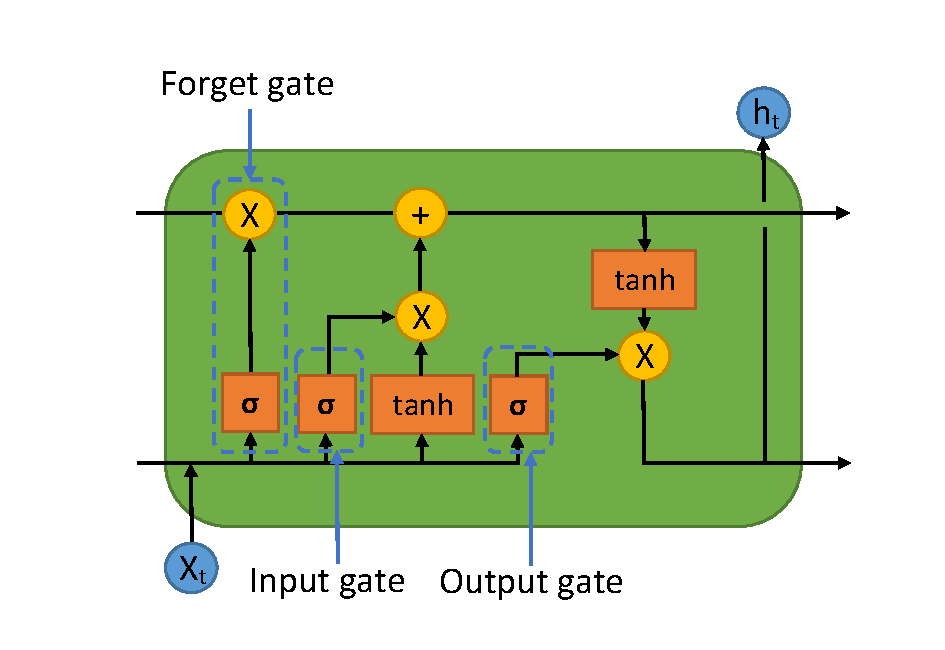
\includegraphics[width=\textwidth]{PICs/temproalModelsSOTA/LSTM.pdf}
        \caption{\ac{LSTM} \cite{LSTM2014}}
        \label{fig:LSTMGRUSOTA_a}
    \end{subfigure}
    \hfill
    % Zweite Grafik (b)
    \begin{subfigure}[t]{0.49\textwidth}
        \centering
        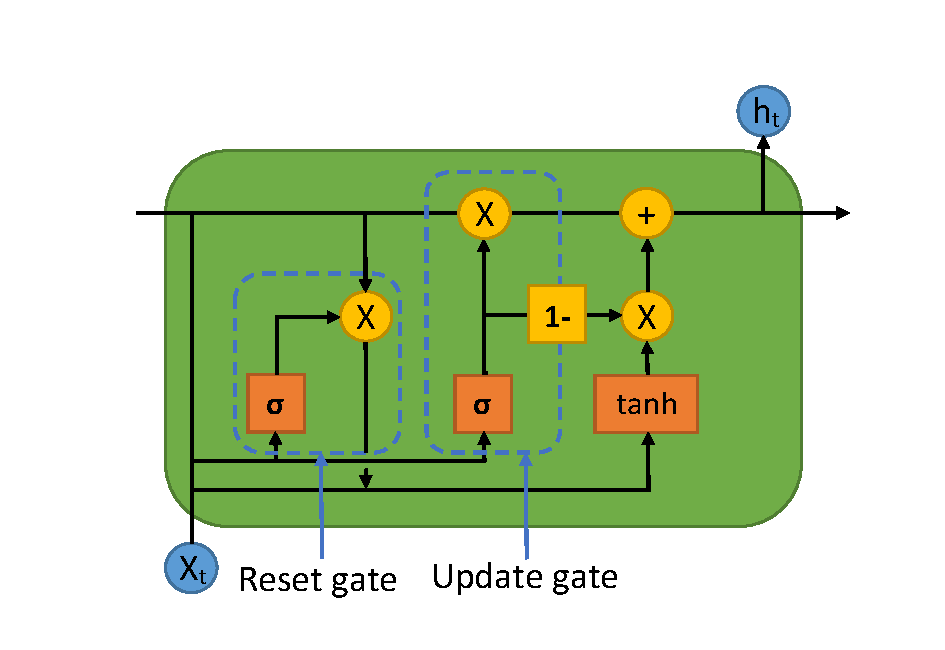
\includegraphics[width=\textwidth]{PICs/temproalModelsSOTA/GRU.pdf}
        \caption{\ac{GRU} \cite{GRU2014}}
        \label{fig:LSTMGRUSOTA_b}
    \end{subfigure}
    \caption{Common \ac{RNN} architectures.}
    \label{fig:LSTMGRUSOTA}
\end{figure}

\noindent Another method to process sequential data can be \ac{SNN}s \cite{spikingNeuralNetworksReview2022}.
Conventional \ac{ANN}s have computational demands and need a large amount of data.
\ac{SNN}s try to counteract these shortcomings by using biologically realistic neurons.
These realistic neurons process information with impulses referred to as spikes.
The functionality of \ac{SNN}s makes them well-suited for integration with temporal data \cite{spikingNeuralNetworksReview2022}.
In addition, they are more energy efficient than typical \ac{ANN}s \cite{spikingNeuralNetworks2019}.
\cite{uNetAsSNN2021} proposes one example of a \ac{CV} task using \ac{SNN}s.
The \ac{ANN}-based U-Net architecture is converted into an \ac{SNN}.
It runs on an Intel Loihi neuromorphic chip \cite{Loihi2018}, a spike-based neuromorphic hardware.
These tailored hardware are often required to fully exploit the advantages of \ac{SNN}s.
Compared to the \ac{ANN}-based technique, the advantage lies in a significantly decreased power consumption \cite{uNetAsSNN2021}.
However, the non-differentiable function and the complex dynamics of \ac{SNN}s are the reason for a limited range of applications in \ac{CV} \cite{spikingNeuralNetworksReview2022} \cite{spikingNeuralNetworks2019}.
Therefore, \ac{SNN}s are not further considered in this work even though they are suited for temporal data handling and show energy-efficient operation.

Different \ac{RNN} architectures that learn from temporal data have been presented.
However, the use case of this work is a \ac{CV} task.
Therefore, using such temporal models solely is insufficient.
A combination of \ac{CNN} and \ac{RNN} must be implemented.

There are different variations to combine these two network types.
They can be implemented in a parallel manner, processing inputs separately and then combining the outputs of both networks with fully connected layers, like the proposed model of \cite{CNNLSTMparallel2021}.
The \ac{RNN} can first process input data, and the output is then processed by a \ac{CNN}, like in \cite{LSTMCNN2022}.
\cite{CNNLSTM2020} introduced another method, where the model utilizes a \ac{CNN} as the backbone and then an \ac{LSTM} for learning spatio-temporal dependencies.

The structure depends heavily on the existing data and the use case for which the model must be tailored.
Of the three different arrangements of networks, the \ac{CNN}-\ac{RNN} \cite{CNNLSTM2020} is most similar to a vision-based rail track prediction system when input data is considered.
\cite{CNNLSTM2020} introduces a deep-learning approach for modal analysis because of various shortcomings when using traditional measuring techniques.
The input is a video of a vibrating structure, and the output is the fundamental modal frequencies.
Experiments show robust and accurate sensing abilities.

More similar use cases in research that use a combination of \ac{CNN}s and \ac{RNN}s are available in the road domain.
These deal with road lane detection and are also examined in this chapter due to their close similarity to the task of this work.

\cite{robustLaneDetection2020} introduced a semantic segmentation approach that outputs a binary mask for road lanes.
The problem formulation is a sequence-to-one.
Therefore, the model inputs a series of images and outputs the prediction for the last frame.
The proposed model architecture is an encoder-decoder network with an \ac{LSTM} module in between.
The encoder extracts features of the images, resulting in a series of feature maps inputted into the \ac{LSTM} module.
The output of the \ac{LSTM} is the decoder's input.
The \ac{GT} is the labeled binary mask of the last image of the sequence.

\clearpage

\noindent\cite{CNNGRU2022} introduced a similar approach.
A sequence-to-one approach is implemented that predicts the road lanes of the last frame and outputs a binary mask.
This project also implements an encoder-decoder network architecture.
Two ConvGRUs are utilized to learn the temporal component.
One is between the encoder and the decoder for high-level relations between frames.
The other is after the second convolutional block of the encoder to capture low-level features.
Additionally, the model incorporates skip connections between encoder and decoder blocks by concatenating feature maps.

The approach of \cite{hybridSTLanedetction2023} segments road lanes with an encoder-decoder architecture that incorporates an \ac{RNN} between the convolutional layers.
Experiments have been conducted with \ac{RNN}s like \ac{LSTM}, ConvLSTM, \ac{GRU}, and ConvGRU.
This model is also built to serve a sequence-to-one formulation that takes in a series of images and outputs a binary mask for the last image.
Additionally, the model incorporates an SCNN module into the encoder.
This module focuses on learning spatial information in four directions within an image: up, down, right, and left. Furthermore, skip connections are added between the encoder and decoder layers that concatenate feature maps.
Experiments show that combining the SCNN module and the ConvLSTM outperforms other variations.

In 2023, \cite{robustLaneDetection2023} proposed a novel strategy for detecting road lanes by exploiting the temporal dimension.
The introduced model architecture is similar to other state-of-the-art architectures with an encoder-decoder network, including a ConvLSTM between its \ac{CNN} components.
However, the main contributions of this paper are a pre-training stage and the use of a customized PolyLoss.
In the pre-training stage, the model tries to rebuild missing pixels from randomly masked images.
After this stage, the weights are used to train the model for segmenting road lanes and output a binary mask.
In this stage, PolyLoss is utilized to calculate weighted errors.
After the model is trained and outputs a binary mask of road lanes, a DBSCAN and Curve fitting are utilized in the post-processing stage.

To conclude this chapter, some key aspects crystallize out of the state-of-the-art.
First, for road lane detection, a sequence-to-one problem formulation is commonly used, in which a series of images are taken as input, and the output is the prediction of the last image of this sequence.
Secondly, using \ac{LSTM}s or variations is widespread and outperforms other \ac{RNN} models.
Like the state-of-the-art single-image networks, an encoder-decoder structure is usually adopted for road lane detection.
An \ac{RNN} module is usually incorporated between these two network parts to learn spatio-temporal dependencies.
Furthermore, an increase in accuracy or robustness is achieved by exploiting the temporal dimension.
